\section{Tutorial: Algoritmos de Dibujo Simples}

Un \emph{algoritmo} es una secuencia precisa de instrucciones que
controla el comportamiento del computador. En este tutorial aprenderás
a dibujar figuras simples usando una plataforma similar a la tortuga
Logo. Logo es un lenguaje de programación desarrollado en la década de
1960 enfocado principalmente para uso educacional. Es una excelente
plataforma para crear algoritmos de dibujo simples.

\subsection{Qué Aprenderás}
En este tutorial aprenderás:

\begin{itemize}

\item A usar comandos de Logo para dibujar figuras simples.

\item A definir procedimientos simples para simplificar el proceso de
  dibujo.

\end{itemize}

Para comenzar, descarga el proyecto \appName{Logo1} desde
\resources{ProgramaTusIdeas/Dia7} e importalo en \AppInventor. Este
proyecto sirve como plantilla que tiene una aplicación ya funcionando
y que te permite usar comandos de dibujo Logo. La~\Cref{fig:Logo1}
muestra la interfaz de usuario de la aplicación.

\begin{figure}[H]
  \centering
  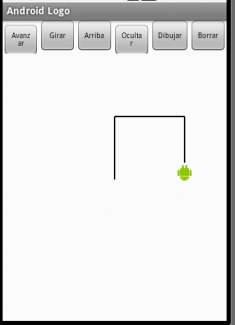
\includegraphics[scale=0.5]{Logo1}
  \caption{Interfaz de usuario Android Logo}
  \label{fig:Logo1}
\end{figure}

Los comandos implementados en los botones son:

\begin{itemize}
\item Avanzar: hace que el Androide avance 10 pixeles.

\item Girar: hace que el Androide gire 90 grados a la derecha.

\item Arriba/Abajo: un interruptor que levanta el lápiz desde el
  lienzo de dibujo (pasa a modo ``no dibujar''), o bien pone el lápiz
  sobre el lienzo (modo ``dibujar'').

\item Ocultar/Mostrar: un interruptor que hace que el Androide
  desaparezca y aparezca.

\item Dibujar: este botón ejecutará cualquier algoritmo que pongas en
  el procedimiento \block{dibujar} como parte de los ejercicios de
  este tutorial.

\item Borrar: este botón borra el lienzo y pone al Androide de vuelta
  al centro del lienzo.

\end{itemize}

Logo es un lenguaje de programación inventado por Seymour Papert en la
década de 1960, principalmente para usos educativos. Papert sostenía
que los estudiantes aprenden mejor cuando están construyendo su propio
conocimiento e ideas. Algo similar pasa en este taller, donde buscamos
que tú Programes Tus Ideas!

El enfoque usado por Papert se conoce como \emph{aprendizaje
  constructivista}, el cual se inspira en la visión de que los
individuos  construyen modelos mentales para entender el
mundo alrededor de ellos. Sin embargo, el constructivismo sostiene que
el aprendizaje ocurre con mayor efectividad cuando las personas están
activas construyendo \emph{objetos tangibles en el mundo real}.

En este tutorial, los \emph{objetos tangibles} que construirás son los
\emph{algoritmos} para dibujar figuras simples.

La característica más conocida de Logo es su tortuga---realmente, un
dibujo de una tortuga--que el usuario puede controlar diciéndole cómo
moverse. A medida que la tortuga se mueve, deja tras de sí un rastro,
o en otras palabras, dibuja al avanzar. Puedes imaginarlo como el
rastro dejado por un animal cuando se mueve por la arena en la
playa. Logo puede usarse para crear algoritmos muy sofisticados, y por
lo tanto dibujos muy sofisticados (Por ejemplo, ver
\url{http://en.wikipedia.org/wiki/Turtle_graphics}).

\subsection*{Comandos Logo}

El lenguaje de programación Logo consiste en un conjunto de comandos
primitivos que controlan a la tortuga. En esta implementación de Logo,
hemos reemplazado la Tortuga por un Androide. Por lo tanto tus
algoritmos le dirán al Androide qué hacer. Además, la versión de este
tutorial está deliberadamente construida con comandos mucho más
``débiles'' que la versión original de Logo. Los comandos que puedes
usar para construir tus algoritmos son:

\newcommand\logoCommand[1]{\textbf{\textit{#1\xspace}}}

\begin{itemize}

\item Comando \logoCommand{Avanzar}: mueve al Androide hacia
  adelante 10 pixeles.

\item Comando \logoCommand{Girar}: hace que el Androide gire 90 grados
  hacia la derecha.

\item Comando \logoCommand{subirLapiz}: sube el lapiz sobre el lienzo
  de manera que nada se dibuja cuando la tortuga se mueve. El comando
  \logoCommand{bajarLapiz} pone el lápiz sobre el lienzo para que se
  vuelva a dibujar.

\item Comando \logoCommand{mostrarTortuga}: hace visible al
  Androide. El comando \logoCommand{ocultarTortuga} hace invisible al
  Androide.

\item Comando \logoCommand{dibujar}: mueve al Androide de acuerdo al
  código que tú especificas. Aquí es donde pondrás tus algoritmos de
  dibujo.

\item Comando \logoCommand{borrar}: limpia el lienzo y mueve al
  Androide de vuelta a la posición inicial al centro del lienzo.

\end{itemize}

Todos estos comandos ya están implementados como procedimientos de
\AppInventor en el proyecto \appName{Logo1} que descargaste e
importaste. Deberías ver que estos bloques están colapsados en el
\blockEditor, como se muestra en la~\Cref{fig:Logo2}.

\begin{figure}[H]
  \centering
  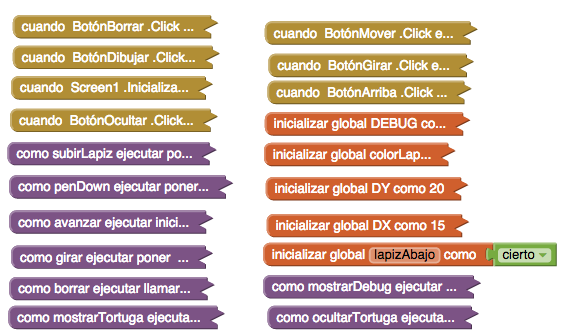
\includegraphics[scale=0.5]{Logo2}
  \caption{Bloques colapsados de los comandos básicos para mover al Androide.}
  \label{fig:Logo2}
\end{figure}

\textbf{No tienes que modificar estos procedimientos} (sí puedes
mirarlos si tienes curiosidad, pero no los cambies!).

\subsection*{Algoritmos}

Un \emph{algoritmo} es una secuencia precisa de instrucciones que,
cuando se ejecutan en un computador, controlan el comportamiento del
computador. Un algoritmo es similar a una \emph{receta de cocina} pero
tiene que ser mucho más preciso que eso si se espera que un computador
la pueda seguir. Las recetas a menudo tienen instrucciones muy
imprecisas que un cocinero novato no sabría cómo hacer. Por ejemplo,
``revuelva hasta que la masa esté suave''. Un cocinero experimentado
podría saber exactamente qué significa eso, pero no todos lo sabrían.

Cada instrucción en un algoritmo debe tener un significado preciso y
no ambiguo. Por ejemplo, la~\Cref{fig:Logo3} muestra un algoritmo para
dibujar un cuadrado de 10 por 10 pixeles en nuestra versión de Logo. A
la izquierda, se expresa el algoritmo en \emph{pseudocódigo} y en la
derecha se muestra como bloques de \AppInventor.

\begin{figure}[H]
\centering
\begin{minipage}{0.5\textwidth}
\centering
\begin{verbatim}
        para dibujar un cuadrado
        de 10 por 10 pixeles:
              avanzar
              girar
              avanzar
              girar
              avanzar
              girar
              avanzar
              girar
\end{verbatim}
\end{minipage}%
%
\begin{minipage}{0.5\textwidth}
  \centering
  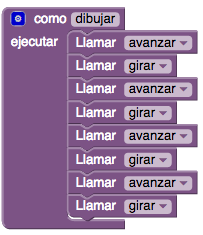
\includegraphics[scale=0.6]{Logo3}
\end{minipage}
  \caption{Algoritmo para dibujar un cuadrado de 10 por 10 pixeles. A
    la izquierda en pseudocódigo, a la derecha en bloques de \AppInventor.}
  \label{fig:Logo3}
\end{figure}

El \emph{pseudocódigo} es un lenguaje para expresar algoritmos que es
muy similar al Español (o Inglés) pero que también incluye código
similar al del computador. Su propósito es proveer una manera
conveniente de expresar algoritmos como \emph{texto}.

\subsection*{Ejercicios}

Usa el botón ``Guardar proyecto como'' para crear distintas versiones
de la aplicación para cada uno de los ejercicios siguientes. Utiliza
una hoja cuadriculada para diseñar los algoritmos de los ejercicios.

\begin{enumerate}

\item Diseña un algoritmo para dibujar un cuadrado de 20 por 20
  pixeles. Observa que \textbf{\textit{diseñar}} un algoritmo
  \emph{no} es lo mismo que \textbf{\textit{programarlo}}. Al
  principio trata de escribirlo a mano o en una pizarra mientras
  trabajas con algún compañero. Parte del diseño es averiguar o
  establecer qué es lo que tu diseño debería hacer---es decir,
  imaginarte a ti mismo como el Androide y seguir los pasos del
  algoritmo para ver cuál es el resultado. También puedes hacer este
  ejercicio con un compañero, tomando turnos para tener el rol de la
  tortuga o Androide.

  Después de que hayas diseñado un buen algoritmo, implementalo en
  \AppInventor modificando el procedimiento \procedure{dibujar} para
  que dibuje un cuadrado de 20 por 20.

\item Ahora usemos un poco de \emph{abstracción}. Una ventaja será que
  puedes guardar todos tus algoritmos para usarlos en ejercicios
  futuros.

  Define un procedimiento llamado \block{cuadrado20} que dibuja un
  cuadrado de 20 por 20 y luego modifica el procedimiento
  \block{dibujar} para que llame a \block{cuadrado20}. Por ejemplo, en
  la~\Cref{fig:Logo4} se muestra la abstracción para el cuadrado de 10
  por 10, que luego se invoca desde \block{dibujar}.

\begin{figure}[H]
  \centering
  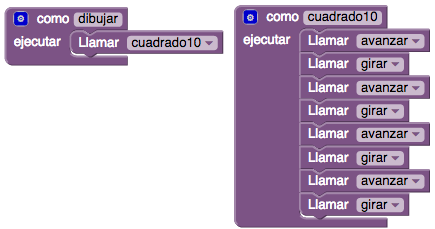
\includegraphics[scale=0.6]{Logo4}
  \caption{Usando abstracción: código para procedimiento
    \block{cuadrado10} y cómo se llama desde el procedimiento
    \block{dibujar}.}
  \label{fig:Logo4}
\end{figure}

\item Diseña un algoritmo para dibujar un cuadrado de 40 por 40
  pixeles. Luego implementa tu algoritmo definiendo el procedimiento
  \block{cuadrado40} que dibuja un cuadrado de 40 por 40
  pixeles. Modifica el procedimiento \block{dibujar} para que llame a
  \block{cuadrado40}.

\item Diseña un algoritmo para dibujar una cara con un cuadrado grande
  para la cabeza, 2 cuadrados pequeños para los ojos, y una línea para
  la boca (la nariz es opcional!). Si necesitas otros procedimietos
  para ayudarte a resolver el problema, diséñalos y defínelos.

\textbf{Diseña primero, y después programa!} Este algoritmo será un
poco más complejo que cualquiera de los anteriores. Tendrás que usar
el procedimiento \block{subirLapiz} para despegar el Androide del
lienzo. También tendrás que planificar cúan lejos moverte hacia
adelante para colocar correctamente los ojos y la
boca. \textbf{Definitivamente querrás planificar y probar este
  algoritmo en papel o en la pizarra antes de intentar programarlo.}

Cuando hayas diseñado un algoritmo correcto, impleméntalo como el
procedimiento \block{dibujarCara} que dibuja una cara. Luego prueba tu
código para asegurarte que lo hiciste todo correctamente.

\item ¿Puedes dibujar un triángulo con el conjunto actual de comandos
  Logo? Discute por qué sí o por qué no.

\item Discute sobre qué necesitaríamos cambiar sobre los comandos Logo
  para poder dibujar un triángulo.

\end{enumerate}

\section{Tutorial: Algoritmos de Dibujo con Repetición y Selección}

En el tutorial anterior desarrollaste algoritmos para dibujar figuras
simples. Sin embargo esto fue difícil porque los comandos que usaste
eran muy débiles e inflexibles. Por ejemplo, el comando
\logoCommand{avanzar} sólo podía usarse para mover al Androide hacia
adelante 10 pixeles. Asímismo, el comando \logoCommand{girar} sólo
podía girar al Androide en 90 grados. Con estos comandos dibujar un
cuadrado de 100 por 100 pixeles sería algo muy
\emph{tedioso}\footnote{Eliminar el tedio y el aburrimiento de hacer
  cosas repetitivas es una gran fuerza motivadora en el desarrollo de
  nuevos algoritmos, lenguajes de programación, \emph{frameworks} y
  \emph{librerías}. En cierto sentido, un programador ``flojo'', en el
  sentido de ahorrar trabajo innecesario, llega a ser un buen
  programador!} y además era imposible dibujar un simple triángulo!

En este tutorial hemos mejorado el conjunto de comandos al
\textit{\textbf{hacerlos más generales}}. Las mejoras principales
están en los comandos \logoCommand{avanzar(N)} y
\logoCommand{girar(G)}:

\begin{itemize}
\item El comando \logoCommand{avanzar(N)} mueve el Androide \textbf{N
    pixeles hacia adelante}.

\item El comando \logoCommand{girar(G)} hace que el Androide
  \textbf{gire G grados hacia la derecha}.

\end{itemize}

Los valores \parameter{N} y \parameter{G} son \emph{parámetros} o
\emph{argumentos}. Un ejemplo sencillo debiera bastar para mostrar por
qué son más general, y por lo tanto, más poderosos. En el tutorial
anterior, para mover el Androide 40 pixeles hacia adelante había que
llamar 4 veces al comando \logoCommand{avanzar}, como se ve en
la~\Cref{fig:Logo5}.

\begin{figure}[H]
\centering
\begin{minipage}{0.5\textwidth}
\centering
\begin{verbatim}
              avanzar             
              avanzar
              avanzar
              avanzar
\end{verbatim}
\end{minipage}%
%
\begin{minipage}{0.5\textwidth}
  \centering
  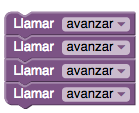
\includegraphics[scale=0.7]{Logo5}
\end{minipage}
\caption{Algoritmo para avanzar 40 pixeles, usando el comando
  \logoCommand{avanzar} en su versión inflexible.}
  \label{fig:Logo5}
\end{figure}

Compara esto con la~\Cref{fig:Logo6} donde,
usando el nuevo conjunto de comandos, basta con una llamada
\logoCommand{avanzar(40)}.

\begin{figure}[H]
\centering
\begin{minipage}{0.5\textwidth}
\centering
\begin{verbatim}
              avanzar(40)
\end{verbatim}
\end{minipage}%
%
\begin{minipage}{0.5\textwidth}
  \centering
  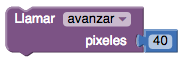
\includegraphics[scale=0.7]{Logo6}
\end{minipage}
  \caption{Algoritmo para avanzar 40 pixeles, usando el comando
  \logoCommand{avanzar} en su versión general.}
  \label{fig:Logo6}
\end{figure}

La primera versión de \logoCommand{avanzar} era muy \emph{específica}
mientras que la nueva versión, con un parámetro, es más \emph{general}
y es precisamente la presencia del parámetro lo que le da su
generalidad. En vez de siempre avanzar 10 pixeles, ahora podemos
avanzar cualquier número de pixeles en una sola llamada al
procedimiento. La misma observación aplica también al procedimiento
\logoCommand{girar}. La abstracción anterior era muy específica,
porque nos dejaba girar sólo 90 grados. La nueva abstracción, al
involucrar un parámetro, nos deja girar cualquier número de grados.

\emph{Nota:} tanto la versión anterior y la actual de los
procedimientos Logo son \emph{abstracciones}. Pero, claramente, el
nuevo conjunto de abstracciones es mucho más poderoso. Como regla
general, mientras más general es un procedimiento o abstracción, es
mejor.

Los otros comandos Logo son los mismos que en la versión anterior:

\begin{itemize}

\item Comando \logoCommand{subirLapiz}: sube el lapiz sobre el lienzo
  de manera que nada se dibuja cuando la tortuga se mueve. El comando
  \logoCommand{bajarLapiz} pone el lápiz sobre el lienzo para que se
  vuelva a dibujar.

\item Comando \logoCommand{mostrarTortuga}: hace visible al
  Androide. El comando \logoCommand{ocultarTortuga} hace invisible al
  Androide.

\item Comando \logoCommand{dibujar}: mueve al Androide de acuerdo al
  código que tú especificas. Aquí es donde pondrás tus algoritmos de
  dibujo.

\item Comando \logoCommand{borrar}: limpia el lienzo y mueve al
  Androide de vuelta a la posición inicial al centro del lienzo.

\end{itemize}

Para comenzar con los siguientes ejercicios, descarga el proyecto
\appName{Logo2} desde la carpeta \resources{ProgramaTusIdeas/Dia7} e
impórtalo en \AppInventor. Al igual que en la versión anterior, hemos
programado todos los bloques requeridos para que entres a programar
tus algoritmos; estos bloques, que se muestran en la~\Cref{fig:Logo7},
están colapsados y no es necesario que
los edites.

\begin{figure}[H]
  \centering
  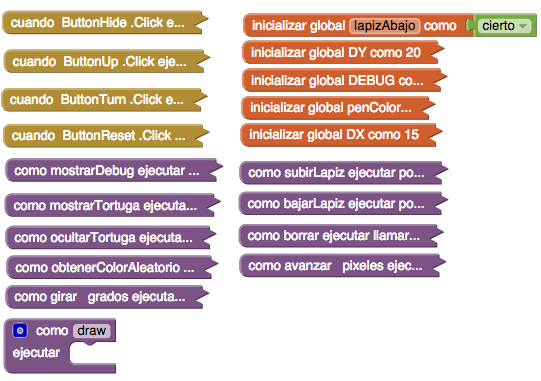
\includegraphics[scale=0.6]{Logo7}
  \caption{Bloques ya programados de la aplicación
    \appName{Logo2}. Nota que hay un nuevo bloque \block{obtenerColorAleatorio}.}
  \label{fig:Logo7}
\end{figure}

\subsection*{Definir un Procedimiento con Argumentos}

En el tutorial anterior definiste procedimientos sin
parámetros, pero pronto necesitarás definir procedimientos con
parámetros. Para hacer esto, necesitas arrastrar un bloque
\block{procedimiento} hacia el área de trabajo. Como siempre, debes
darle un nombre adecuado a tu procedimiento. Luego, para especificar
que el procedimiento requiere un parámetro cuando es llamado, presiona
el botón azul y arrastra un bloque \block{entrada x} desde la
izquierda, hacia los bloques de la derecha (similar a como agregas una
condición \block{si no}, a un bloque condicional). Observa
la~\Cref{fig:Logo8} para ver cómo tiene que ser.

\begin{figure}[H]
  \centering
  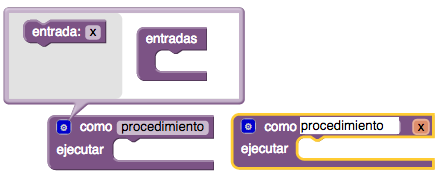
\includegraphics[scale=0.6]{Logo8}
  \caption{Creando un procedimiento con parámetros.}
  \label{fig:Logo8}
\end{figure}

Reemplaza el nombre del parámetro, \parameter{x}, con un nombre más
útil y significativo. Puedes agregar más parámetros si es necesario;
una vez que termines de agregar parámetros presiona nuevamente el
botón azul.

\subsection*{Algoritmos con Repetición y Selección}

Al diseñar algoritmos hay tres tipos básicos de \emph{estructuras de
  control}: secuencias, selección y repetición. Cualquier algoritmo
que puedas imaginar puede construirse con estos tres tipos de control.

\paragraph{Secuencias} Ya estás familiarizado con las secuencias, que
simplemente significan una secuencia de pasos. En \AppInventor ponemos
los bloques en secuencia al apilar unos sobre otros, como se ve en
la~\Cref{fig:Logo9}.

\begin{figure}[H]
  \centering
  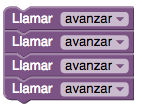
\includegraphics[scale=0.6]{Logo9}
  \caption{Una secuencia de llamadas a \block{avanzar}.}
  \label{fig:Logo9}
\end{figure}

\paragraph{Selección} También estás familiarizado con la selección,
que es simplemente un término que usamos para estructuras
\block{si-sino}, por ejemplo como se ve en la~\Cref{fig:Logo10}.

\begin{figure}[H]
  \centering
  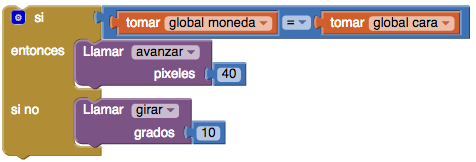
\includegraphics[scale=0.6]{Logo10}
  \caption{Un bloque usando selección.}
  \label{fig:Logo10}
\end{figure}

\paragraph{Repetición} Hasta ahora no hemos usado \emph{repetición} (o
\emph{looping} en inglés) en nuestros algoritmos. La~\Cref{fig:Logo11}
muestra un ejemplo simple de cómo un loop puede ser muy útil. Compara
los algoritmos a la izquierda y a la derecha.

\begin{figure}[H]
\centering
\begin{minipage}{0.5\textwidth}  
 \centering
  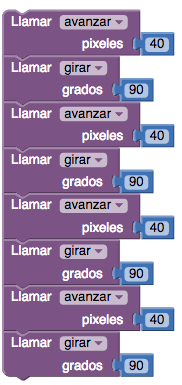
\includegraphics[scale=0.7]{Logo11a}
\end{minipage}%
%
\begin{minipage}{0.5\textwidth}
  % \centering
  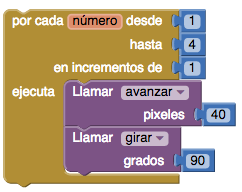
\includegraphics[scale=0.7]{Logo11b}

\paragraph{Cómo leer este bloque:}
Para cada \parameter{número} (el contador del loop) desde 1 hasta 4,
incrementando cada paso en 1, ejecuta los bloques dentro de
``ejecuta''. Por lo tanto el \parameter{número} cambiará a 1, 2, 3 y
4.

En otras palabras, repite los bloques dentro de ``ejecuta'' 4 veces.
\end{minipage}
  \caption{Ejemplo de un algoritmo que usa repetición.}
  \label{fig:Logo11}
\end{figure}

El algoritmo a la izquierda usa una secuencia simple con copias de las
llamadas a \block{avanzar} y \block{girar} para dibujar un
cuadrado. Por otro lado, el algoritmo a la derecha utiliza un loop
\block{por cada}; lo que es un enfoque mucho más práctico y
general. En este caso, el bloque \block{por cada}
\textbf{\emph{repite}} los bloques dentro de ``ejecutar'' 4 veces. Hay
muchos usos para este bloque, pero por ahora veremos un uso
sencillo. Muchos de los ejercicios de este tutorial pueden programarse
usando el loop como se muestra aquí: contando desde \block{inicio}
hasta \block{fin}, con incrementos de 1 en 1.

En el ejemplo de la~\Cref{fig:Logo11} colocamos valores constantes
para los valores de inicio, fin, e incremento. Pero también puedes
poner variables! Por ejemplo, la~\Cref{fig:Logo12} muestra un
procedimiento que dibuja una estrella un poco rara, como la de
la~\Cref{fig:Logo13}.

\begin{figure}[H]
  \centering
  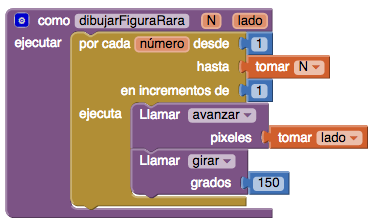
\includegraphics[scale=0.6]{Logo12}
  \caption{El procedimiento \block{dibujarFiguraRara} que usa una
    variable \variable{N} en un loop.}
  \label{fig:Logo12}
\end{figure}

\begin{figure}[H]
  \centering
  
\includegraphics[scale=0.6]{Logo13}
  \caption{Una figura dibujada al llamar a
    \block{dibujarFiguraRara}. ¿Qué argumentos debes usar para obtener
    esta figura?.}
  \label{fig:Logo13}
\end{figure}

Copia el procedimiento \block{dibujarFiguraRara} y empieza a jugar con
el número de repeticiones. ¿Cuántas repeticiones necesitas para
dibujar una estrella completa?'

\subsection*{Ejercicios}

\begin{enumerate}

\item Usando un bloque \block{por cada} define un algoritmo para
  dibujar un cuadrado, de nombre \block{dibujarCuadrado(L)}, que
  dibujará un cuadrado de tamaño $L \times L$ donde $L$ es el largo
  del lado.

\paragraph{Nota Importante!} En \AppInventor y otros lenguajes de
programación, los parámetros pueden tener \emph{cualquier} nombre. Por
lo tanto es importante usar nombres que describen el propósito del
párametro. Esto hará que leer el código sea más fácil para ti y para
otros programadores. Por ejemplo, compara los nombres en
la~\Cref{fig:Logo14}.

\begin{figure}[H]
  \centering
  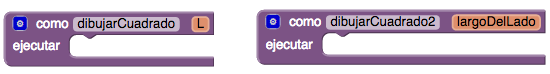
\includegraphics[scale=0.6]{Logo14}
  \caption{Una comparación sobre nombres de parámetros.}
  \label{fig:Logo14}
\end{figure}

\item Diseña un algoritmo para dibujar un triángulo equilatero. Es
  decir, un triángulo donde los lados y los ángulos son
  iguales. Primero diseña el algoritmo a mano---¿cuanto tiene que girar
  el Androide?

  Este ejercicio es un ejemplo de una repetición, así que puedes usar
  el bloque \block{por cada} en tu algoritmo. ¿Cuántas repeticiones
  son necesarias?

  Una vez que tengas diseñado tu algoritmo, impleméntalo en
  \AppInventor y pruébalo. Define el algoritmo como un procedimiento
  con 1 parámetro, para que así lo puedas reutilizar en el futuro si es
  necesario. ¿Qué debe representar el parámetro?

\item Dibuja un pentágono, es decir, una figura de 5 lados donde los
  lados y los ángulos son iguales. Sigue el proceso del ejercicio
  anterior. Este ejemplo también es un ejemplo de repetición, así que
  usa el bloque \block{por cada}. ¿Cuántas repeticiones son
  necesarias?

\paragraph{Pista:} para dibujar un cuadrado, el Androide tiene que
girar 4 veces en 90 grados, lo que significa que en total gira 360
grados.

Una vez que tengas listo tu algoritmo, impleméntalo como un
procedimiento de 1 parámetro. ¿Qué depresenta este parámetro?

\item Los cuadrados y pentágonos son ejemplos de una figura más
  general, que se conoce como \emph{polígono}. Un polígono es una
  figura con múltiples lados. Por lo tanto, un cuadrado es un polígono
  con 4 lados, y un pentágono es un polígono con 5 lados. Si pudieras
  diseñar un procedimiento \block{dibujarPolígono(N,L)}, entonces podrías
  usarlo para dibujar un cuadrado, un pentágono, un hexágono (6
  lados), un octágono (8 lados), o incluso una aproximación de un
  círculo (¿36 lados?). Inténtalo!

  \paragraph{Pista:} Tu procedimiento necesitará 2
  parámetros, \parameter{N} y \parameter{L}, donde \parameter{N} es el
  número de lados (por ejemplo, 4, 5, 6, etc) y \parameter{L} es el
  largo de cada lado.

\paragraph{Pista:} Un cuadrado tiene 4 lados y sus giros son en
$360/4$ grados. Un pentágono tiene 5 lados y sus giros son en $360/5$
grados. Un hexágono... . Un $N$-ágono...

Prueba tu procedimiento \block{dibujarPolígono(N,L)} usándolo para dibujar un
hexágono y un octágono. Conecta el nuevo bloque dentro del bloque
\block{dibujar} para que cuando el usuario presione el botón
``Dibujar'' se ejecute tu algoritmo.

\item Usa \block{dibujarPolígono(N,L)} para dibujar un círculo. Este
  ejercicio puede requerir mucho ensayo-error para obtener el número
  correcto de lados y el largo de los lados. ¿Un polígono de 36 lados
  se parece a un círculo?

\item Para dibujar una flor, dibuja repetidamente un cuadrado y luego
  gira algún número de grados. Por ejemplo, ve
  la~\Cref{fig:Logo15}. Para cambiar el color del lápiz debes cambiar
  la propiedad \property{Lienzo.ColorDePintura}. Puedes usar el
  procedimiento \block{obtenerColorAleatorio} que ya viene provisto
  para obtener colores al azar.

\begin{figure}[H]
  \centering
  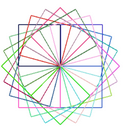
\includegraphics[scale=0.6]{Logo15}
  \caption{Una flor dibujada mediante repeticiones de dibujar un
    cuadrado y luego girar.}
  \label{fig:Logo15}
\end{figure}

\item Dibuja una flor a la que le falten algunos pétalos, como en la~\Cref{fig:Logo16}. Para ello
  utiliza una moneda (es decir, elige un número aleatorio entre 0 y 1)
  para tomar la decisión de dibujar o no algún cuadrado.

\begin{figure}[H]
  \centering
  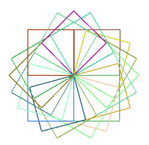
\includegraphics[scale=0.6]{Logo16}
  \caption{Una flor a la que le faltan algunos pétalos.}
  \label{fig:Logo16}
\end{figure}

\item Diseña y dibuja tus propias figuras, incluyendo flores,
  espirales, estrellas, etc. Por ejemplo, la flor de
  la~\Cref{fig:Logo17} se hizo dibujando círculos y girando.

\begin{figure}[H]
  \centering
  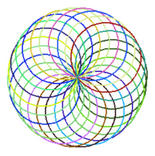
\includegraphics[scale=0.6]{Logo17}
  \caption{Una flor en base a círculos.}
  \label{fig:Logo17}
\end{figure}

\end{enumerate}

\section*{Resumen}

La lección principal aquí es que la elección de nuestras
abstracciones, en este caso el uso de parámetros en los comandos Logo,
afecta la clase de problemas que podemos resolver y cómo los
resolvemos. Es decir, nuestra elección en cuanto a abstracción tiene
un enorme impacto en nuestros algoritmos. Además, la abstracción
procedural (con y sin parámetros) facilita la construcción de
algoritmos al elevar el nivel de abstracción.

Si te gustó jugar con la programación, te recomendamos que veas el
sitio \url{https://blockly-games.appspot.com/} donde hay juegos en
línea basados en bloques de código muy similares a los de \AppInventor!










